\documentclass[12pt]{article} 
\usepackage{geometry} %页边距设置等

%-----------------------------format.tex-----------------
\usepackage{amsmath,amssymb} 
\usepackage{float}
\usepackage{graphicx}
\usepackage{fancybox}
\usepackage{fancyhdr} 
\usepackage{lastpage}
\usepackage{hyperref}
\hypersetup{
    unicode={true},pdfstartview={FitH},pdfborder={0 0 0},
    colorlinks,linkcolor=black,citecolor=black,hyperindex,plainpages=false,}   %目录超链接格式设置
% style: page layout
\setlength{\headheight}{15pt}
\setlength{\headsep}{20pt}
\setlength{\footskip}{30pt}
\setlength{\voffset}{-5pt}
\setlength{\hoffset}{16pt}
\setlength{\oddsidemargin}{0pt}
\setlength{\evensidemargin}{\oddsidemargin}
\setlength{\marginparpush}{0pt}
\setlength{\marginparwidth}{0pt}
\addtolength{\textheight}{3\baselineskip}

% Definitions的格式设置
\newtheorem{definition}{{definition}}
\newcounter{numdefinition}
\renewenvironment{definition}[1]
{\noindent\stepcounter{numdefinition}
\slshape Definition \arabic{numdefinition} \textsf{#1 :}
\begin{quote}\small\itshape}
{\end{quote}}

\newcommand{\dd}{\ensuremath{\,\mathrm{d}}}
%===============================================================
\fancypagestyle{plain}%重新定义plain格式,用于summary sheet
{\fancyhf{}
\setlength{\headheight}{0pt}\setlength{\headsep}{0pt}
\setlength{\voffset}{-50pt}\setlength{\oddsidemargin}{0pt}}

%===============================================================
\graphicspath{{pic/}}

%=========================定义页眉===============================
\pagestyle{fancy} 
\lhead{page\thepage\ of \pageref{LastPage}}
\chead{} \rhead{Team \footnotesize{\#} 666} \lfoot{}
\cfoot{\thepage}
\rfoot{}
\renewcommand{\headrulewidth}{0pt}
\setcounter{secnumdepth}{3}
\begin{document}

%=========================summary sheet.tex========================

\thispagestyle{empty}
\begin{minipage}{0.3\textwidth}
\begin{flushleft}
For office use only\\
   T1\ \rule{3cm}{0.5pt}\\
   T2\ \rule{3cm}{0.5pt}\\
   T3\ \rule{3cm}{0.5pt}\\
   T4\ \rule{3cm}{0.5pt}\\
\end{flushleft}
\end{minipage}\hspace{\fill}
\begin{minipage}{0.3\textwidth}
\centering
Team Control Number\\[5pt]
\fontsize{36pt}{\baselineskip}\selectfont  \textbf{666} \normalsize\\[10pt]
Problem Chosen\\[5pt]
\fontsize{18pt}{\baselineskip}\selectfont \textbf{A }\normalsize\\
\end{minipage}\hfill
\begin{minipage}{0.35\textwidth}
\begin{flushright}
\shortstack[l]{
For office use only\\
   F1\ \rule{3cm}{0.5pt}\\
   F2\ \rule{3cm}{0.5pt}\\
   F3\ \rule{3cm}{0.5pt}\\
   F4\ \rule{3cm}{0.5pt}}
\end{flushright}
\end{minipage}\vspace*{10pt}
\rule{\textwidth}{0.5pt}

\begin{center}
  \textbf{2016 Mathematical Contest in Modeling (MCM) Summary Sheet}
\end{center}
%\enlargethispage
\noindent
{\Large \textbf{Abstract}}
\vspace{7pt}

%==========================abstract.tex==============================
We have constructed a Stability time series model and a Markov model that to hold a promise for providing insight into not only predict the max ozone hole square in Antarctic in the next 50 years, but also foresee the ozone levels in different latitudes in the northern hemisphere in the next 50 years. This model considers a large number of parameters thought to be important to the ozone hole and ozone levels, including the CSCs concentration, the destruction CFCs to the ozone layer, light intensity, the atmospheric circulation, solar radiation and temperature. 

The aforementioned Stability time series approach includes CFCs concentration data (1979-2016), max ozone hole square data in Antarctic (1979-2016) and the average solar radiation in Antarctic each year, in order to research the relationship between the max ozone hole square and the CFCs concentration and predict the max ozone hole square in the later 50 years by using the Holt-Winters Method. 

The Markov model approach includes the ozone levels data of $15\,^{\circ}N$ to $55\,^{\circ}N$ in the northern hemisphere in 1986 to 2016. Ozone transition, impacting the ozone levels in different latitudes and the CFCs concentration. The different day length in the different latitudes determined the reaction time of CFCs and the ozone. The day length, CFCs concentration and ozone transition can be reflect in the historical changes. We get the probability transfer matrix from the historical data, which can predict the most probable ozone levels in the $15\,^{\circ}N$ to $55\,^{\circ}N$.

Specific attention is given to the sensitivity of our model to variations in its fundamental parameters, whose values are based largely on inadequate and varied statistical data. We attempt to use our model to identify the most important factors related to the ozone levels, and show simulation results related to α in the Stability time series model.

Ultimately, we have concluded that given the complex nature of this scenario and the limited quantity and quality of detailed information concerning the change of max ozone hole square in Antarctic and the ozone levels in the $15 \,^{\circ}N$ to $55\,^{\circ}N$ in the next 50 years, it is not possible at this time to quantitatively predict the effectiveness of the ozone levels recovery plan. Instead, the results presented here qualitatively show the relationship between ozone hole square and CFCs concentration .These qualitative results are then used to craft a tentative deployment strategy for the ozone levels recovery.
%\textbf{keyword}: sweet spot; corked bat; coefficient of restitution;%xxx speed; finite element method; 
\newpage

%====================目录页========================================
\thispagestyle{empty}
\setcounter{page}{0}
{\begin{center}\Large \textbf{The Model of Ozone Level Prediction in 50 Years}\end{center}}
\tableofcontents                                                  %
\newpage                                                          %
%==================================================================

\newcommand{\vw}{\frac{v_i}{\omega_i}}

%=======================\input{introduction1}=======================
\section{Introduction}
\subsection{Context of The Problem}

The ozone layer protects Earth from dangerous UV radiations which can cause mutations . In humans, higher rates of skin cancers, cataracts, and immune system problems can be the consequences of the damage of ozone layer. Furthermore, an increase in UV radiation could affect plants and marine ecosystem. thus gives the earth a constant influence. 

\begin{center}
\begin{figure}[htpb]
\centering
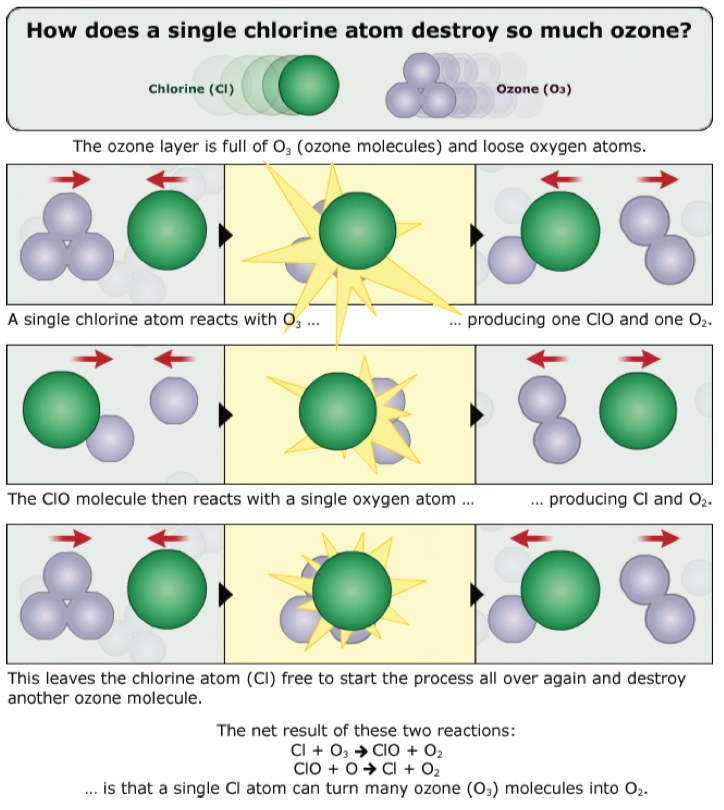
\includegraphics[scale=0.8]{Formular}
\caption{Formular}\label{fig:Formular}
\end{figure}
\end{center}

By the studies of F.Sherwood Rowland and Mario Molina, the ozone layer is full of $O_3$ (ozone molecules) and loose oxygen atoms, once a single atom reacts with $O_3$ it will producing one $ClO$ and one $O_2$,but the $ClO$ molecule won't stay long, soon it will react with a single atom and finally producing $Cl$ and $O_2$. This reaction will start to process all over and over again, destroy a huge amount of ozone molecules.

Later in Rowland, Solomon, and Garcia’s work, another modified version of the original hypothesis was suggested. It shown that noting will affect CFCs in the lower atmosphere, and  the CFCs will eventually diffuse to the upper atmosphere releasing $Cl$ atoms when exposed to solar radiation. Also, nitrogen dioxide neutralizes some $Cl$ in upper atmosphere. This will speed up the depletion of ozone. In the meantime, these scientist find that this process  goes much more faster with the help of the polar clouds, due to the Ice particles speed release of chlorine and keep nitrogen dioxide from neutralizing much more chlorine.

These studies revealed the reasons why ozone hole could appear and why it mainly happens over the Antarctic.

\begin{center}
\begin{figure}[htpb]
\centering
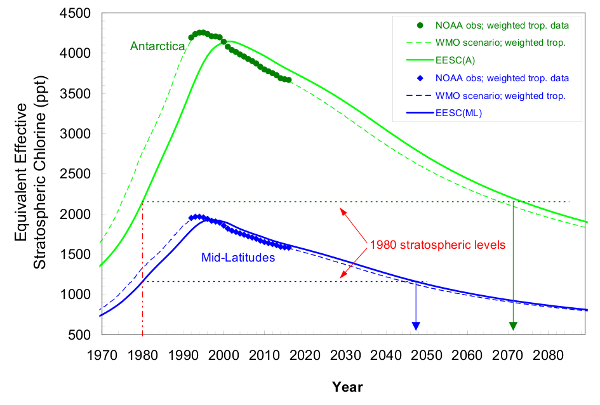
\includegraphics[scale=0.8]{cfc}
\caption{CFCs Level}\label{fig:CFCs Level}
\end{figure}
\end{center}

\begin{center}
\begin{figure}[htpb]
\centering
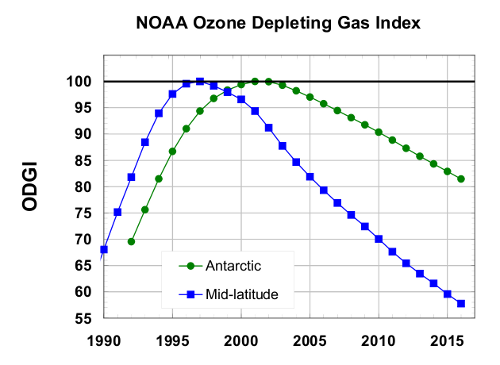
\includegraphics[scale=0.9]{cfc_index}
\caption{CFCs Index}\label{fig:CFCs index}
\end{figure}
\end{center}



In 1985, 20 nations signed the Vienna Convention for the Protection of the Ozone Layer. In 1987, representatives from 43 nations signed the Montreal Protocol. At Montreal, the participants agreed to freeze production of CFCs at 1986 levels and to reduce production by 50 percent by 1999. Since the adoption and strengthening of the Montreal Protocol has led to reductions in the emissions of CFCs, atmospheric concentrations of the most-significant compounds have been declining.   Besides, the factors that influence the ozone content and change in the atmosphere also include the light intensity, the atmospheric circulation and eddy transport. The equator is the most likely region to produce ozone, which receives the strongest solar radiation, but due to the role of atmospheric circulation, the ozone generated will be brought to the north and south. The polar vortex causes the wind blowing to the north and south to be less, thus stopping the exchange of material there. Because of the destruction to the ozone layer by contaminants, the ozone layer is gradually consumed, but there are no ozone supplement from outside area , so the content will be significantly reduced.
\subsection{Finding The Data}
Scientists use various method to collect the ozone area and other data. For example, in order to get the data of ozone levels in different level, high-altitude balloons with sensitive measuring devices were flew into the upper atmosphere.

But use balloons to collect data would be like trying to detect a single drop of dye in an Olympic-sized swimming pool full of water. So NASA started using satellite to collect the data. But at first, the program written by NASA's staff mistakenly judged the giant change of ozone level as instrument's malfunctions and overlooked them. A few years later, by comparing with the data from ground-based observatories, they finally find the fact that the ozone hole is rapidly expand in a more faster way than anyone can ever imagine.
\begin{center}
\begin{figure}[htpb]
\centering
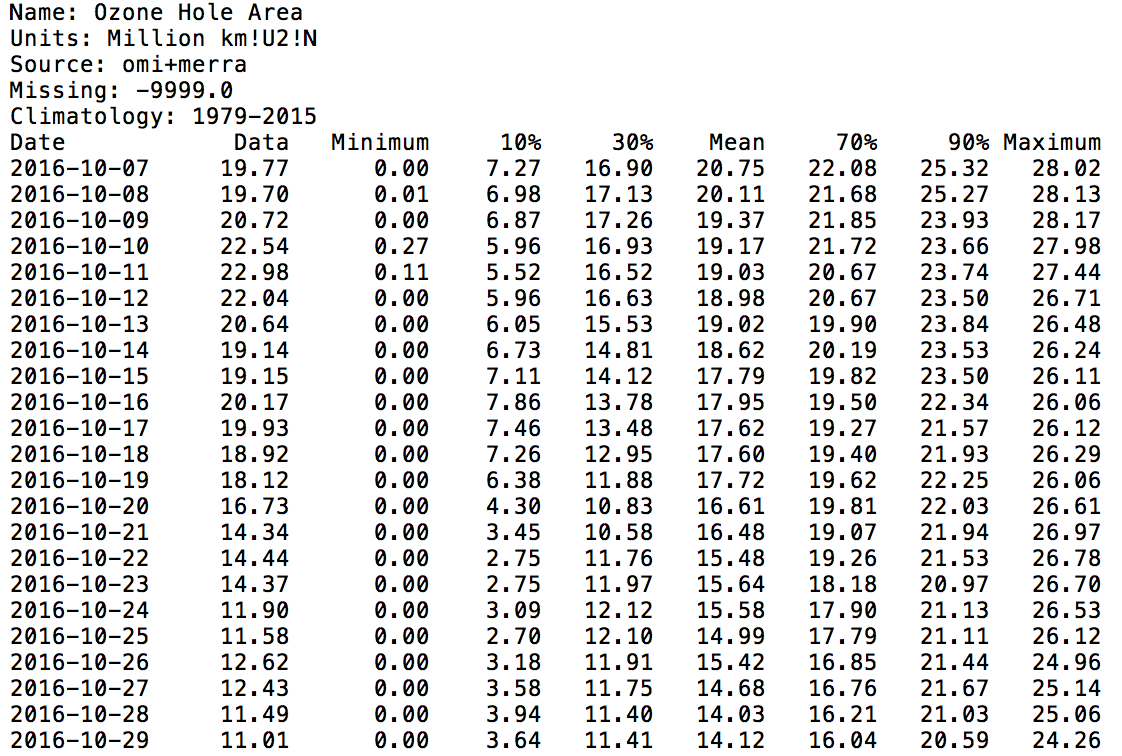
\includegraphics[scale=0.6]{oz_area_data}
\caption{One Ozone hole area data-set example}\label{fig:data}
\end{figure}

\begin{figure}[htpb]
\centering
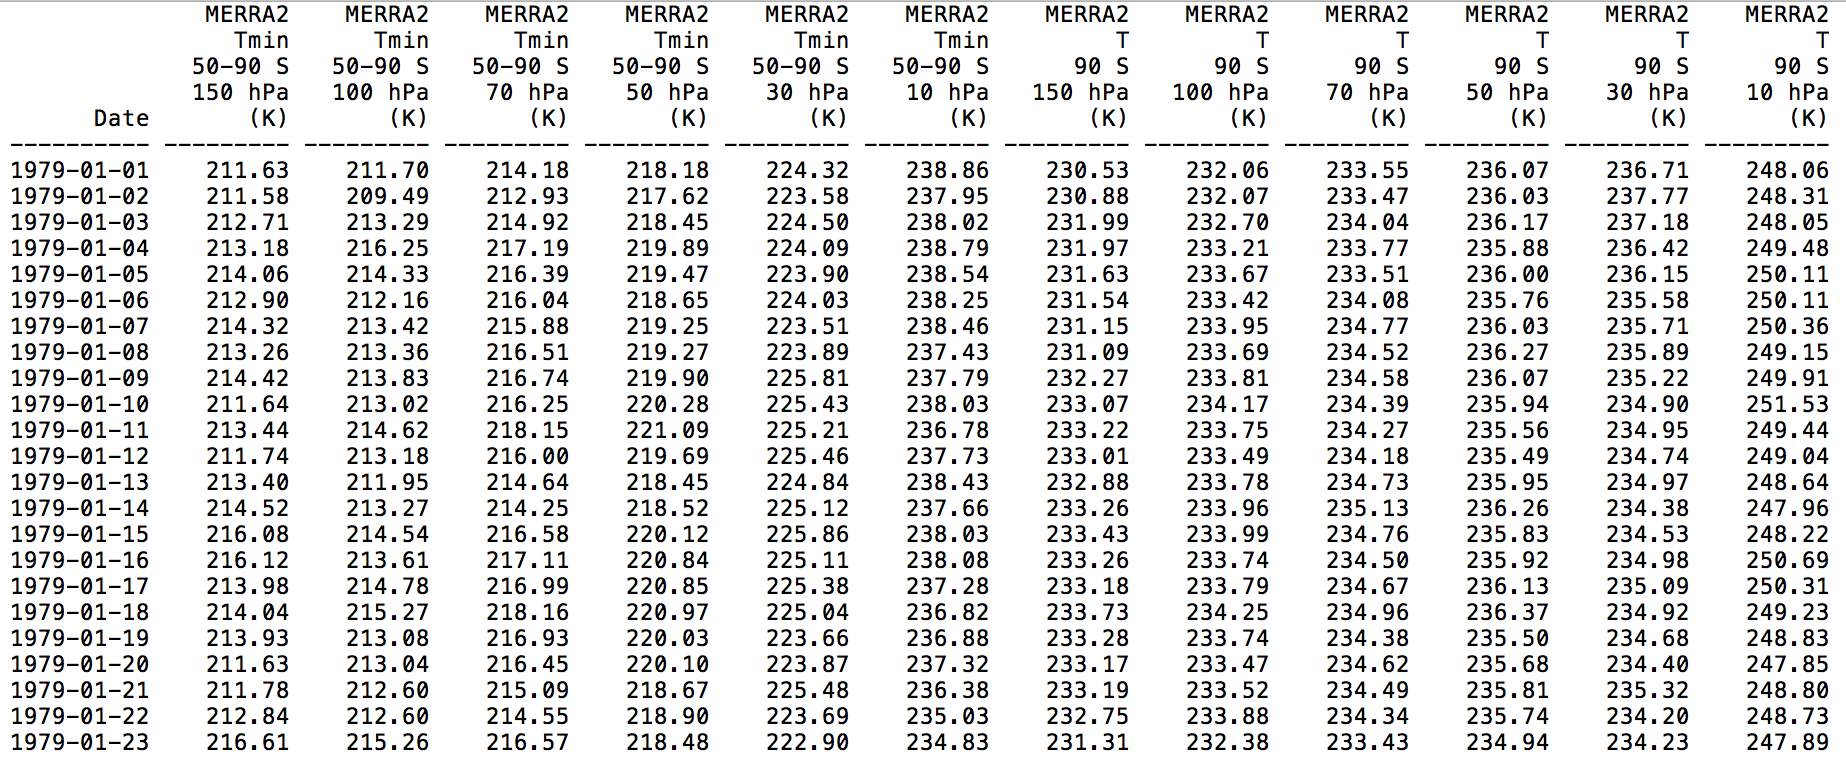
\includegraphics[scale=0.4]{T&T_data}
\caption{One Minimum Temperature data-set example}\label{fig:data}
\end{figure}
\end{center}
The data we used to analysis and predicting the ozone level is a sub-set of NASA's Ozone Data Set, including the everyday's ozone hole area from the year 1979. And the data we find in the NOAA's website indicated the changes of CFCs.
\subsection{Data Preprocessing}
For the data set has some missing data in some days, in order to lowest the mean error, we use the mean value of corresponding  every single data missing day in the past 30 years. And after all the processes we finally got the clean data for further calculating as well as predicting. 

Also, for the ozone levels fluctuate so wildly that it is difficult to detect subtle trends over a short-term period. We use the mean value of each year's ozone hole area as a factor indicate the ozone level thus we can predict the ozone level  in a larger scale.
%img here
\subsection{The Task at Hand}
We should develop a mathematical model to analysis the changes of ozone level and find out the factor of the ozone changes.  For we already know the CFCs' changing patten, we also should analysis the relationship between them and use it for better predicting the ozone level as well as given instructions on CFCs' production and usage.
\subsection{Previous work}
\begin{center}
\begin{figure}[htpb]
\centering
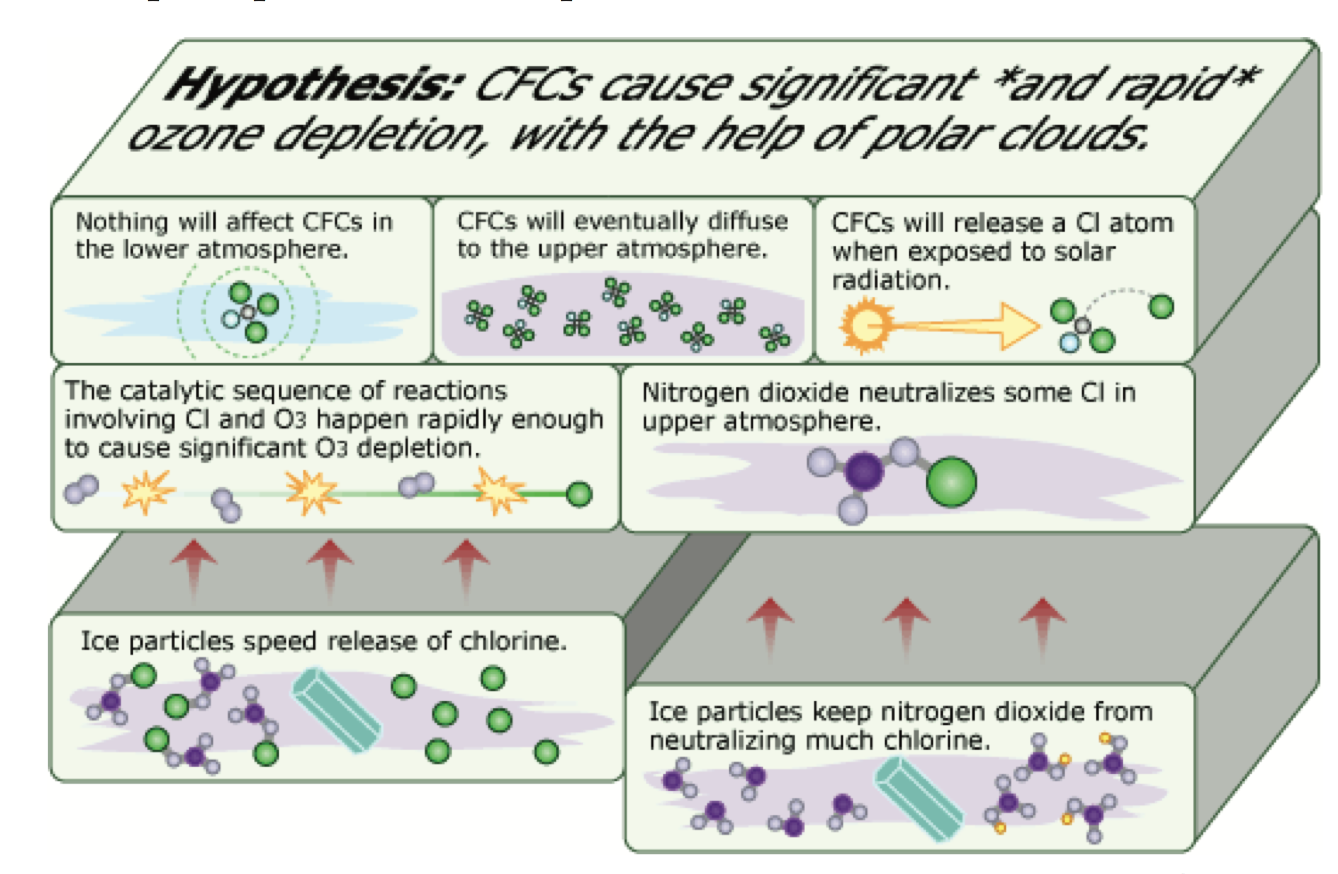
\includegraphics[scale=0.4]{previouswork}
\caption{Rowland, Solomon, and Garcia’s work suggested a modification to the original hypothesis: CFCs cause significant ozone depletion—and they do it much more rapidly with the help of polar clouds.}\label{fig:Formular}
\end{figure}
\end{center}
Scientist use models as one important method to doing research. Modeling often means creating a mathematical model -  a set of equations that represent a real system. 
\begin{center}
\begin{figure}[htpb]
\centering
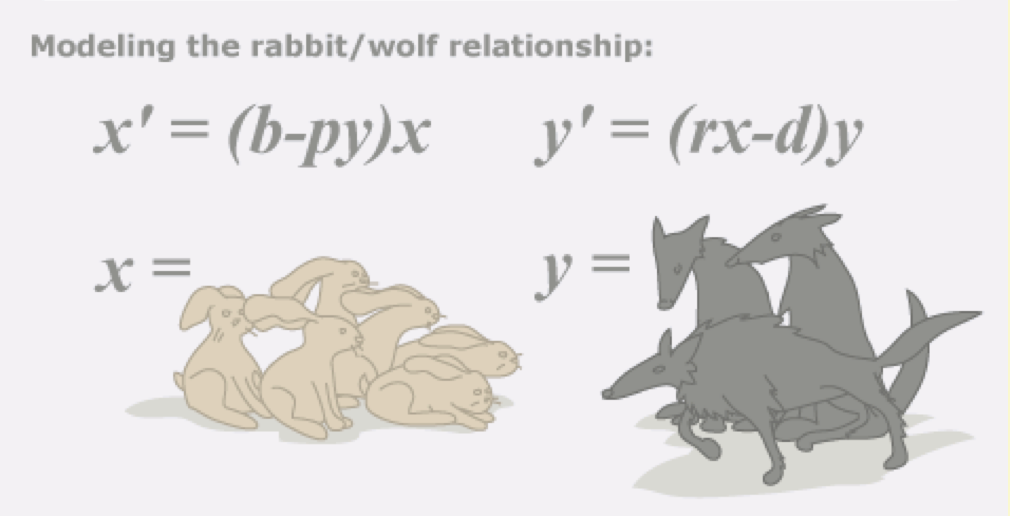
\includegraphics[scale=0.6]{wolf}
\caption{The Wolf Hunting Model to predict the interrelationships.}\label{fig:wolf}
\end{figure}
\end{center}

In the 1970s, scientists tried to us the wolf-rabbit model to predict some interchanges relationships include the CFCs and  The wolf-rabbit model is essentially a hypothesis about the two species and how these interaction affect their numbers. 

And the models and hypotheses about how molecules interact with one another as they move through the atmosphere. Models, and the hypotheses within them, are supported when the model generates expectations that match the behavior of its real-world counterpart—e.g., if removing hunting from the model has a similar effect to that observed in the real world when wolves are protected from hunting . If a model is supported and seems to be a good representation of the real world, we can use it to answer “what if” questions: What would happen to rabbit populations if we allowed wolf hunting in particular areas—or more pertinently for Molina and Rowland, what would happen in 50 years if we continued CFC production at 1974 rates?



%============================\input{definitions1}===========
\section{Definitions}
\begin{definition}{ }
  
\end{definition}

\begin{definition}{}

\end{definition}

\begin{definition}{}

\end{definition}

%=======================\input{Assumptions1}=====================================
\section{Assumptions}
\begin{enumerate}
\item 
\item 
\end{enumerate}

%=====================\input{symbols}==========================================
\section{Symbols}

\begin{tabular}{ll}
\hline
Symbols&Definitions\\
\hline
$t$& time\\
$S_{t+1}$& predicted value of the maximum area of the ozone hole in the year of t+1\\
$S_t$& predicted value of the maximum area of the ozone hole in the year of t\\
$Y_t$& measurement of the maximum area of the ozone hole in the year of t\\
$\alpha$& weighting coefficient\\
$DU$&Dobson Unit, the unit of ozone content\\
$O(t)$& predicted function of the maximum area of the ozone hole\\
$C(t)$& predicted function of CFCs content level\\
$E_i$& the range for ozone content in the state of t\\
$P$& transition probability matrix\\
$P^k$& the transition probability matrix after the year of k\\
$p_{ij}$& the chance to change from the state of $E_i$ to $E_j$\\
$Y$& ozone content\\
\hline
\end{tabular}


%=============================\input{ModelforCollision}==========================
\section{Time series model}
\begin{center}
\begin{figure}[htpb]
\centering
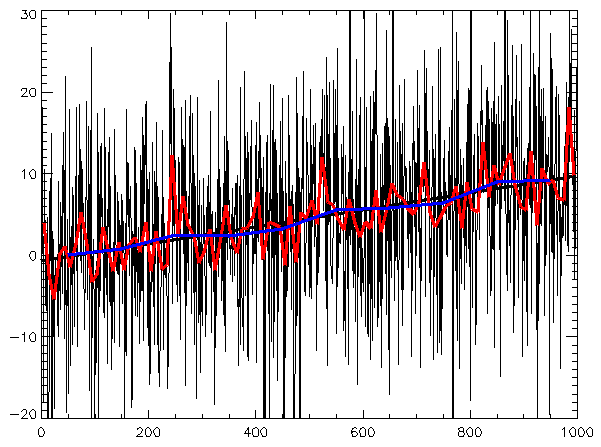
\includegraphics[scale=0.35]{ts_model}
\caption{Time series: random data plus trend, with best-fit line and different applied filters.}\label{fig:ts_exam}
\end{figure}
\end{center}
A time series is a series of data points indexed (or listed or graphed) in time order.Time series analysis comprises methods for analyzing time series data in order to extract meaningful statistics and other characteristic of the data. In our model, we use time series forecasting as the model to predict future ozone level based on previous observed values. While regression analysis is often employed in such a way as to test theories that the current values of one or more independent time series affect the current value of another time series.

Time series data have a natural temporal ordering. This makes time series analysis distinct from other analysis methods.  A stochastic model for a time series will be more closely related than observations further apart. In addition. 

Time series analysis can be applied to real- valued, continuous data, dis Crete numeric data, or discrete symbolic data (i.e sequences of characters).

In our model, we developed a new method to use our data collected from NASA's satellites. The data include informations of daily ozone hole area values(unit: million square  kilometers), and the mean value of corresponding time in the past 30 years.

\subsection{\ Holt-Winters Method \\(Three Order Exponential Smoothing)
}


When the time series have a quadratic feature, we tend to use the Holt-Winters Method to smoothing. Holt-Winters Method takes into account seasonal changes as well as trends(all of which are trends). Seasonality is defined to be the tendency of our time series data that  changes  annually, we  smoothed the changes to be well predictable. While we can use it to predict the future changes.

The method calculates a trend line for there data as well as seasonal indices. $\{S_t^{(1)}\}$ represent the smoothed value of the constant part for time t. $\{S_t^{(2)}\}$ represents the sequence of second value. And the $\{S_t^{(3)}\}$ is the *Three Order Exponential Smoothing Value*. The method is given by the formulas 

\begin{eqnarray}
\left\{
\begin{array}{ll}
 S^{(1)}_t=\alpha y_t+(1-\alpha)S_t^{(1)}  \  , \\
 S^{(2)}_t=\alpha S^{(1)}_t +(1-\alpha)S_{t-1}^{(2)} \  ,\\
 S^{(3)}_t = \alpha S^{(3)}_t +(1-\alpha)S^{(3)}_{t-1}\ ,
\end{array}\right.\label{equ:dynamicofcollision}
\end{eqnarray}

 In the formulas above, $S^{(3)}_t$ is the Three Order Exponential Smoothing Value.And the Holt-Winters Method's prediction model is
$$
\hat y_{t+m} = a_t + b_tm + C_t m^2, (m = 1,2,...)
$$

The parameters are defined as follows

\begin{eqnarray}
\left \{
  \begin{array}{ll}
  a_t = 3S_t^{(1)} - 3S_t^{(2)} +S_t^{(3)}, \\
  b_t = \frac{\alpha}{2(1-\alpha)^2}[(6-5\alpha)S_t^{(1)} - 2(5-4\alpha)S_t^{(2)}+(4-3\alpha)S_t^{(3)}], \\
  c_t=\frac{\alpha^2}{2(1-\alpha)^2}[S_t^{(1)}-2S_t^{(2)}+S_t^{(3)}].
 
\end{array} \right .
\end{eqnarray}
%三次平滑的定义式



\subsection{Trajectory Analysis}
\subsubsection{Comparation}
We get the function of the change of the max Ozonehole square (O(t)) and the function of the change of the total amount of CFCs(C(t)), and draw the two functions in the same cartesian axis. The picture(填个编号)shows how the max Ozone hole square changes with the CFCs concentration. Wesucceed finding that the Ozone hole square reaches the maximum values after theCFCs concentration reaches the maximum values. It means that the increase of Ozone hole square lags behide the increase of CFCs concentration.
Oin which the path taken during the compression phase
is different from that taken during the expansion phase. The area bounded by the two curves is the energy dissipated
\begin{center}
\begin{figure}[htpb]
\centering
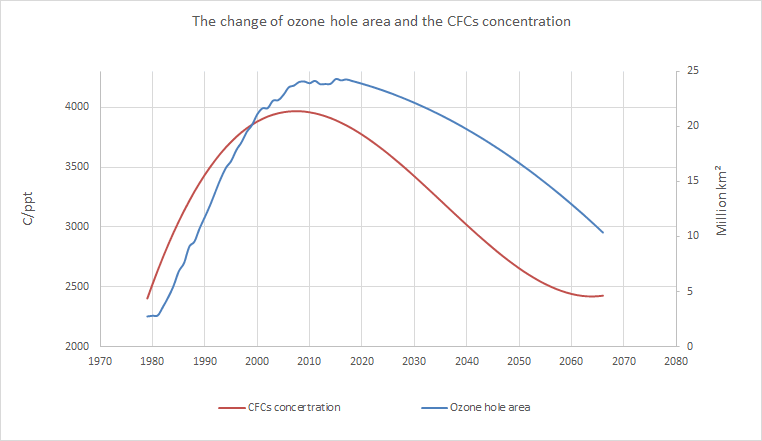
\includegraphics[scale=0.6]{ha}
\caption{}\label{fig:twoline}
\end{figure}
\end{center}
\subsubsection{Trajectory analysis}
In order to researchthe relationship between Ozonehole square and CFCs concentration, we use phase trajectory to analysis the character of function O(t) and C(t), and wedraw the max ozone hole square image on the change of CFCs concentration.
\begin{center}
\begin{figure}[htpb]
\centering
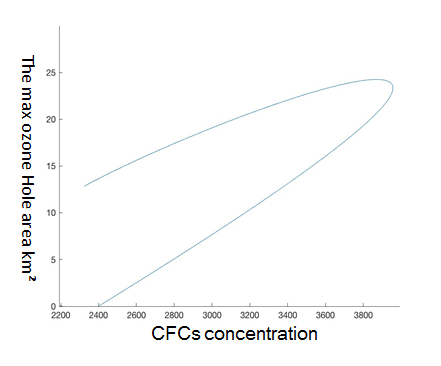
\includegraphics[scale=0.8]{tl}
\caption{Trajectory Analysis}\label{fig:xgx}
\end{figure}
\end{center}
Because of the CFCs concentration increase with the decrease of slope, so wecan judge that the function curve moves counterclockwise.After the CFCs reaches the maximum,the max Ozone hole also reaches the maximum. Because some developed anddeveloping countries sign the Montreal Protocol, the CFCs concentration become lower. However, the production rate of ozone in nature ismuch more slowly than the depletion rate of ozone caused by a great quantity ofCFCs concentration for the reason that ozone only be produced in nature bychemical reactions such as lightning. So phase trajectory does not fall in accordance with theoriginal curve. It decline above the original curve with the increase of slope. But the max ozonehole square in the next 50 years can not return to the level of 1979.

\subsection{Sensitivity Analysis}
Prediction modeling, like ozone levels prediction. To better characterize the sensitivity of our model to the natural variations and errors present in the parameter α which depends on the historical data. We have performed a simulation to find the best parameter to predict the ozone level in the next 50 years.
\begin{center}
\begin{figure}[htpb]
\centering
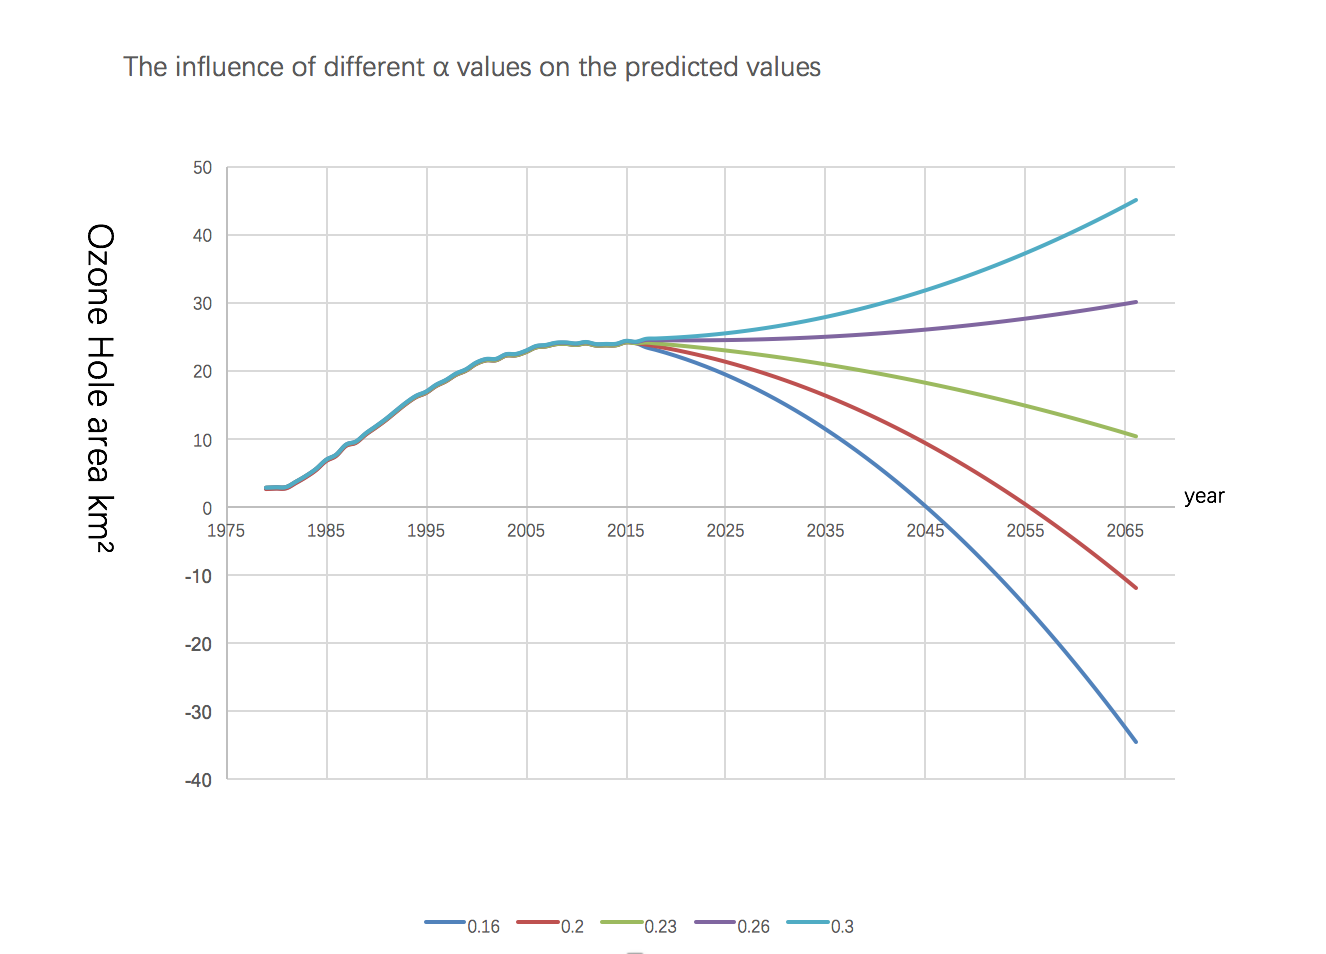
\includegraphics[scale=0.6]{ts}
\caption{Trajectory Analysis Results}\label{fig:xgxfx}
\end{figure}
\end{center}
According to practical experience, α range from 0.1 to 0.3 is appropriate. The parameter α plays control to participate in the average historical data. The greater the α, the less data is used. Take six different values (0.16, 0.2, 0.23, 0.26, 0.3) for α and draw the different prediction curves in on the same axis.
\subsection{Additional Considerations}
\subsection{Strengths and Weaknesses}

\subsubsection{Strengths}
\begin{enumerate}
\item The data we find is widely accepted in society so our results have a higher credibility.
\item Through the stability time series model we are able to predict the max ozone hole square in Antarctic in next 50 years, enabling us to transform an abstract problem into a mathematical one.
\item Through the predicted images, we can clearly list out the data and results, making our work easy to understand.
\item By involving a trajectory analysis, we research the relationship between max ozone hole square and CFCs concentration. We can succeed making the conclusion that the CFCs concentration and the max ozone hole square has the close contact.
\item By involving a sensitivity analysis our model has a better adaptation to environment and we can know that in what situation it is still effective.
\end{enumerate}
\subsubsection{Weaknesses}
\begin{enumerate}
\item We just take the CFCs concentration in to consideration so the model need to be altered because the light intensity also ozone hole square in the Antarctic.
\item We only consider objective data but do not consider some subjective factors, such as how the human will limit the emissions of CFCs in the future.
\end{enumerate}


\section{Markov Model}
\subsection{Prediction Models}
From data of NASA, in 1963 to 1985, the ozone content in atmosphere fluctuate randomly, and there are individual points fluctuate wildly. The ozone content in other years change smoothly, so we can believe that the change satisfies the Markov property approximately(shown below).

From data we found, the observation precision of these data is generally from $±2\%$  to $ ±3\%$, so we can divide into three to five states in states partition by the range for ozone content. If we divide into five states:$$E_1, E_2, E_3, E_4, E_5$$ so every state has five directions to changes:$E_i \to E_1$, $E_i \to E_2$, $E_i \to E_3$, $E_i \to E_4$, $E_i \to E_5 \ \ (i=1,2,3,4,5\ldots)$, we use state transferring probability to describe these changes. The most basic part of state transferring probability is one step transition probability $P\{E_i\to E_j\}$,  written $P_{ij}=P\{E_i\to E_j\}\ \ (i, j=1,2,3,4,5\ldots)$.
When sample size is large enough, we can use example distribution to describe  theoretical distribution of state approximately, so we can use frequency to replace transferring probability between corresponding states. 
We align state transferring probability $P_{ij}=P\{E_i\to E_j\}$ in proper order and get a matrices of order five:
$$
\begin{bmatrix} &E_1&E_2&E_3&E_4&E_5\\E_1&P_{11}&P_{12}&P_{13}&P_{14}&P_{15}\\E_2&P_{21}&P_{22}&P_{23}&P_{24}&P_{25}\\E_3&P_{31}&P_{32}&P_{33}&P_{34}&P_{35}\\E_4&P_{41}&P_{42}&P_{43}&P_{44}&P_{45}\\E_5&P_{51}&P_{52}&P_{53}&P_{54}&P_{55} \end{bmatrix} \quad
$$
In it, $P_{ij} \geq 0$, $\sum_{j=1}^{n}P_{ij}=1 (i=1,2,3,4,5 \ldots)$
    If the current forecasting object is in state$ E_i$, $P_{ij} (i,j=1,2,3,4,5\ldots)$ describes the possibiliy that current $ E_i$ state change into every state, and the most likely situation is the result we predict. In this way, we can get the mostly likely state that forecasting object change into by one step.
Let $P^{(k)}$ be a k-step transition probability matrix, so $P^{(k)}=P^k$
Let A be a matrix, if there is a positive integer m, let $A^m=a_{ij}$ satisfy $a_{ij}>0$ and $$\sum_{j=1}^{n}a_{ij}=1$$ 
So $A$ is a standard probability matrix.
If an one-step transition probability matrix is a standard probability matrix, it must have steady state。
Let $S^{(k)}$ be state vector of forecasting object at time of t=k, so when $$S^{(k)}=S^{(k-1)}P$$ at steady state $$S^{(k+1)}=S^{(k)}$$
Let $$S^{(k)}=(x_1,x_2,……,x_n)=X^{'}$$ and $$\sum_{i=1}^{n}x_{i}=1$$
From formula (1), $S^{(k)}P=S^{(k)}$, we can get $$(P^{'}-E)=0$$ in which the transpose of $X$ is $X^{'}$, while the transpose of $P$ is $P^{'}$.
By solving equations of

\begin{eqnarray}
\left\{
\begin{array}{ll}
(P^{'}-E)X=0 \  , \\
\sum_{i=1}^{n}X_{i}=1\ ,
\end{array}\right.\label{equ:dynamicofcollision}
\end{eqnarray}
we can get $S^{(k)}$, probability of steady state. 

\subsection{Model Implementation}
From the data, we can divide the ozone levels of $15^{\circ}N - 55^ {\circ}N$ into $E_1$,$E_2$,$E_3$,$E_4$,$E_5$ (Table 1).

\begin{center}
\begin{table}[H]
	\caption{Ozone level Prediction of Different Height in 50 Years}\label{tab:thi}
\begin{center}
\begin{tabular}{llllll}
\hline
    ${Latitude \, (^{\circ})} / {value}$ & 15 & 25 & 35 & 45 & 55 \\
\hline
$E_1$ & 245-249 & 251-255 & 299-302 & 313-320 & 320-328\\
$E_2$ & 250-254 & 256-260 & 303-306 & 321-328 & 329-336\\
$E_3$ & 255-259 & 261-265 & 307-310 & 329-336 & 337-344\\
$E_4$ & 260-264 & 266-270 & 311-314 & 337-343 & 345-352\\
$E_5$ & 265-268 & 271-276 & 315-319 & 344-350 & 353-360\\
\hline
\end{tabular}
\end{center}
\end{table}
\end{center}
%===========================================================

Combined with table and data, we can obtain the probability transition matrix $$P_1, P_2, P_3, P_4, P_5$$ The ozone concentration levels of $15^{\circ}N - 55^ {\circ}N$in 2016 are $$E_4, E_3, E_4, E_4, E_1$$ So we can predict the ozone concentration levels of $15^{\circ}N - 55^ {\circ}N$ in 2017 to 2066 will most likely to be by calculating the $P_i^j$ ($i$ from 1 to 50, $j$ from 1 to 5).

\begin{center}
\begin{table}[H]
	\caption{Ozone level of Different Height}\label{tab:thi}
\begin{center}
\begin{tabular}{llllll}
\hline
    $Latitude \, (^{\circ})$ & 15 & 25 & 35 & 45 & 55 \\
\hline
Ozone level (DU) & 254-259 & 266-270 & 303-306 & 329-336 & 337-344\\
\hline
\end{tabular}
\end{center}
\end{table}
\end{center}


\subsection{Strengths and Weaknesses}
\subsubsection{Strengths}
\begin{enumerate}
\item The data we find is widely accepted in society so our results have a higher credibility.
\item Through Markov model we are able to analysis the relationship between the ozone levels and the latitudes, enabling us to transform a abstract problem into a mathematical one.
\item Through figures and tables, we can clearly list out the data and results, making our work easy to understand.
\end{enumerate}
\subsubsection{Weaknesses}
\begin{enumerate}
\item We just take the historical data and the latitudes in to consideration so the model need to be altered because the light intensity and the atmospheric circulation also influence the ozone levels in different latitudes.
\item We only consider objective data but do not consider some subjective factors, such as CFCs emissions are mainly concentrated in the Northern Hemisphere.
\end{enumerate}



%=====================================


\section{Conclusion}
\subsection{Future Ozone Level Trajectories}
An interesting result of our model is that, in the current conditions, the ozone level will recover to around the 1979's level after about 5 to 6 decades. Indeed, a defining characteristic of our model is that the total area of the ozone hole as well as the CFCs content has a relationship with a tiny delay. That means once the CFCs usage or the production has a obvious decline, the ozone hole's area will follows. 
As the Ozone levels fluctuate so wildly but in the meantime they keep the trend of around one particular mean value, that it is difficult to detect subtle trends over a short-term period, but we can say that the ozone level will not get a huge difference. 

While we can also see that the ozone level have a obvious relationship with latitude, in higher latitude, the ozone level comes higher, as the consenquence of the temperature and light. 

Ultimately, we can say that acroding to our model, the ozone level will have a strong relationship with the CFCs or other ozone depleting  gases. And will recover to the level of 1970s by the human-being's action like policy aimed at cutting down the emission of the ozone depleting gases. 

Using  the Markov model, we can also say that prediction that the ozone level in the future 50 years most probably in a given range which given by the table follows.
%==========================表格=============================




%图号
%插图:figure :$v_f$ varies by $z_k$.
%========================Bibtex
\newpage
\bibliography{baseballref}%放在|begin{document}前不可用
\bibliographystyle{ieeetr}%引用格式 ieeetr
%\fi
%\end{CJK}

\end{document}
